\paragraph{Testing methods.} The test data is composed of four
distinct datasets:
\begin{enumerate}[A.]
    \item A simulated dataset similar to the training dataset (14 different individuals, 1008 images)
    \item A small annotated set of plants from real Arabidopsis thaliana (4 different individuals, 6 images);
    \item A larger set of real Arabidopsis thaliana for qualitative evaluation (12 different indivudals, 864 images);
    \item A set of real images from another plant (tomato) to evaluate the possibility of transfering the learning onto other species of plants (TODO).
\end{enumerate}
All datasets will be available there: TODO.

Evaluation is done both on the 2D segmentation and on the resulting segmented 3D point cloud. For datasets A and B,
we present a class by class quantitative evaluation of the 2D segmentation method. For dataset A, we additionally  provide
class by class quantitative evaluation of the 3D voxel segmentation, as well as a comparison of output point clouds
to the ground truth given by L-Py. For dataset C, we provide qualitative assessment of the results of the segmentation,
both in 2D and in 3D. For dataset D, we restrict ourselves to qualitative evaluation of the 2D segmentation.

The background class is not considered as a class in itself in the evaluation, but is presented in the qualitative example. It
is only used for contrast when reconstructing point cloud from voxel data.

\paragraph{2D Segmentation and 3D Segmentation on dataset A.}
Images from datasets A are segmented used the trained neural network. Then, the results of 2D segmentation are
compared to the ground truth provided by the blender simulation. Figure~\ref{fig:seg2d_res} presents a sample from
dataset A and its segmentation.

\begin{figure}
    \centering 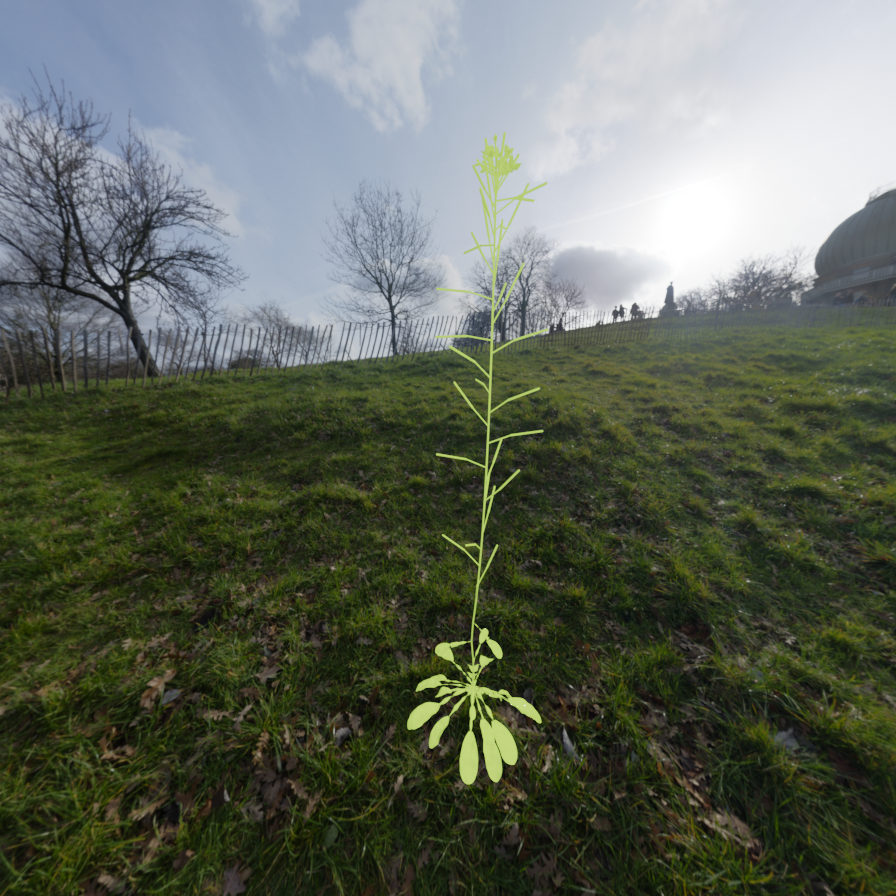
\includegraphics[width = 0.25\linewidth]{figures/00000_rgb.png}\quad
    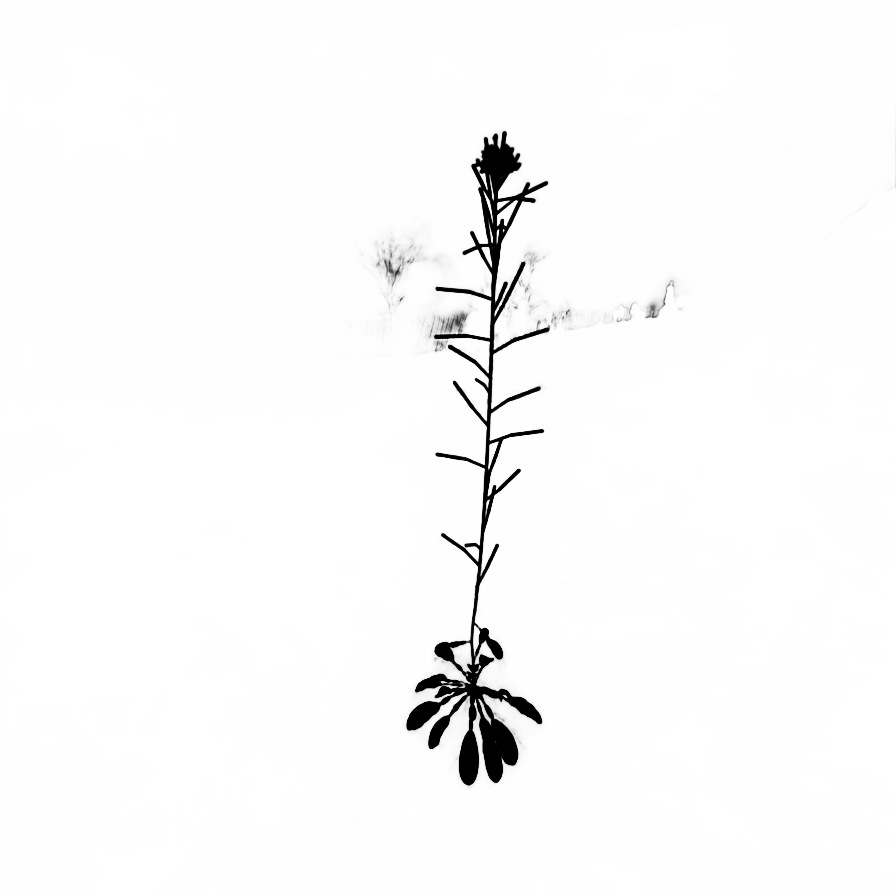
\includegraphics[width = 0.25\linewidth]{figures/000_background.png}\quad
    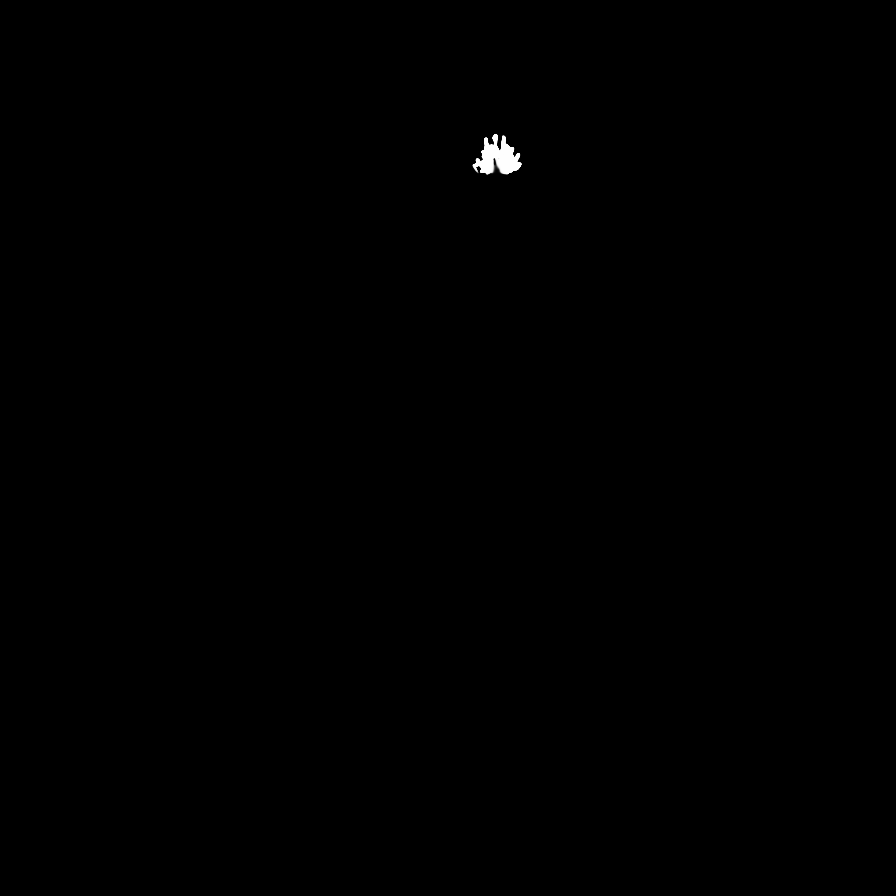
\includegraphics[width = 0.25\linewidth]{figures/000_flower.png}

    \vspace{1em}

    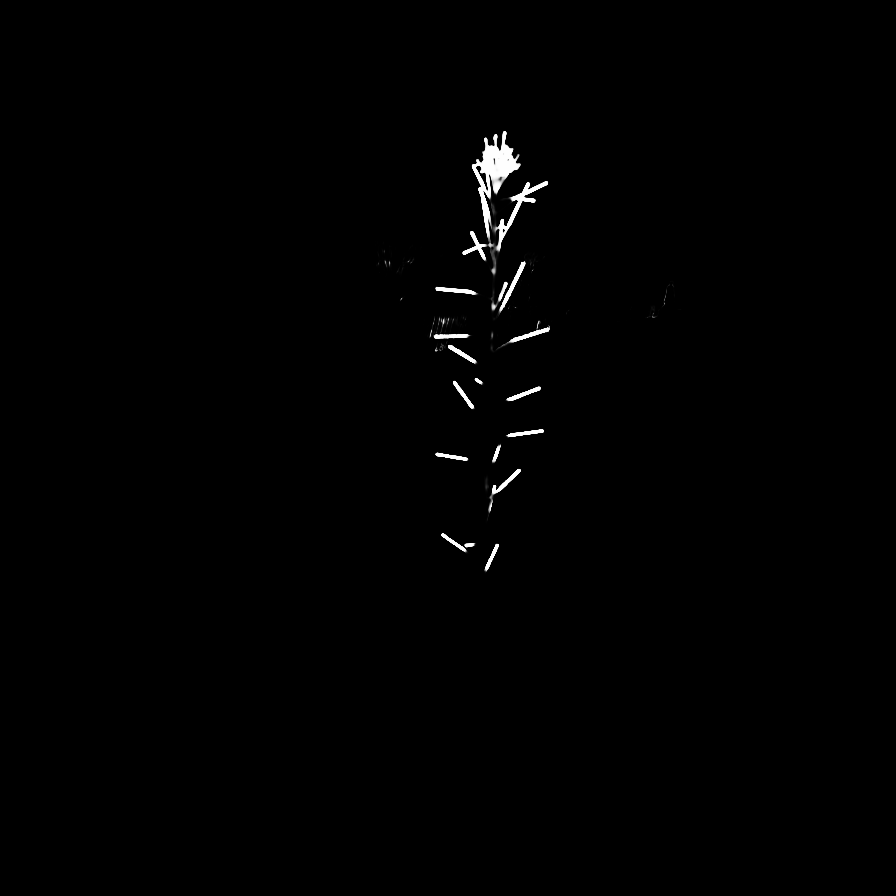
\includegraphics[width = 0.25\linewidth]{figures/000_fruit.png}\quad
    
\includegraphics[width = 0.25\linewidth]{figures/000_leaf.png}\quad
    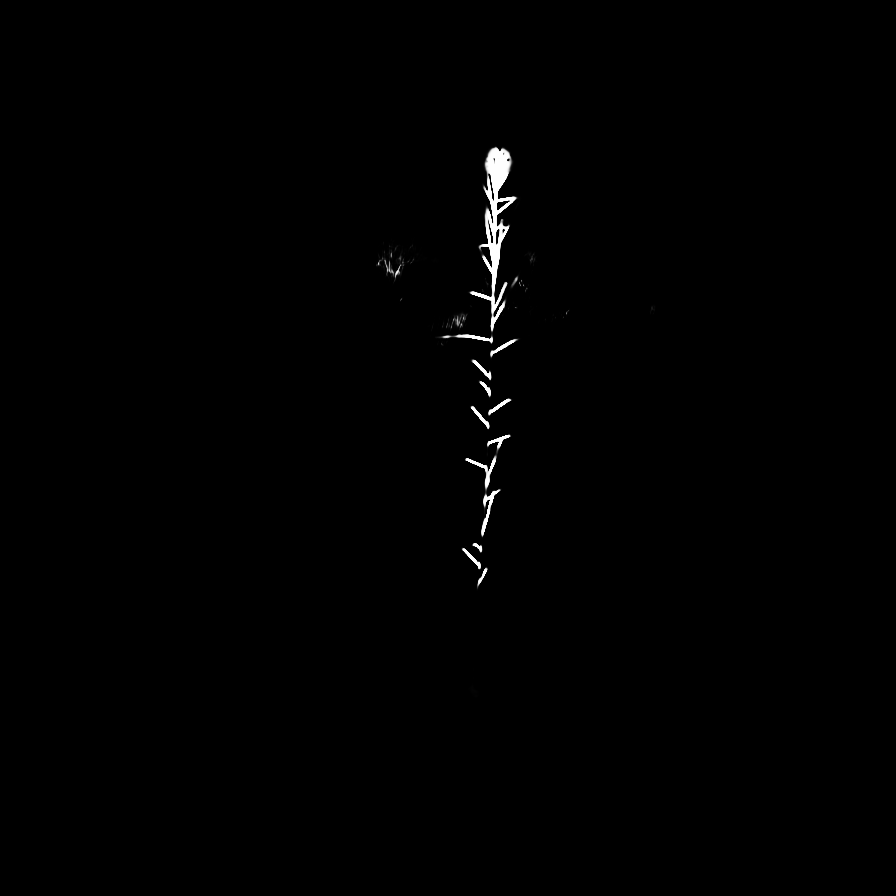
\includegraphics[width = 0.25\linewidth]{figures/000_pedicel.png}
    \caption{Images segmented with our network. From left to right, then top to bottom: original image,
        background, flower, fruit, leaf, pedicel. White indicates a high score (1.0) for the class,
        black indicates a low score (0.0).} \label{fig:seg2d_res}
\end{figure}

Pixels are classified using a threshold on the output of the segmentation
network: for each class $k$, if the score of a pixel is $>0.5$, then the pixel is
positively attributed to class $k$. Given the high contrast of the output images
from the neural netork, the chosen threshold does not matter much. Every pixel
$x$ in then attributed to one of four sets, as classical in the litterature:

\begin{itemize}
    \item $x$ belongs to $\textrm{TP}$ (true positive) if our predicted class is positive and the actual class is
positive;
    \item $x$ belongs to $\textrm{TN}$ (true negative) if our predicted class is negative and the actual class is
negative;
    \item $x$ belongs to $\textrm{FP}$ (false positive) if our predicted class is positive and the actual class is
negative;
    \item $x$ belongs to $\textrm{FN}$ (false negative) if our predicted class is negative and the actual class is
positive;
\end{itemize}

For voxels, the same classification is applied and each voxel is attributed a single class
from the segmentation algorithm presented above, and its class is compared to
the class of the closest point on the mesh produced by L-py.

For both pixels, and voxels, precision and recall are defined as follows and
used as a metric for the accuracy of segmentation:

$$
    \textrm{precision} = \frac{\textrm{\# TP} }{\textrm{\# TP} + \textrm{\# FP}},
    \textrm{recall} = \frac{\textrm{\# TP} }{\textrm{\# TP} + \textrm{\# FN}},
$$

Precision is the proportion of the predicted class which is correctly labeled,
recall is the proportion of all elements of a class which have been predicted.
Figure~\ref{fig:prec_recall_2d_3d} present precision and recall for each class
for both 2D and 3D segmentation. Voxels and pixels are accumulated over all of
dataset A. These results show that precision is roughly equal or slightly better
for almost all classes in 3D than in 2D, but recall suffers on classes which are
occluded a lot: some parts of the stem and some flowers on the top of the plant
models are occluded by pedicel and fruits on almost all pictures, which explains
why some part of it are missed.

\begin{figure}
    \centering 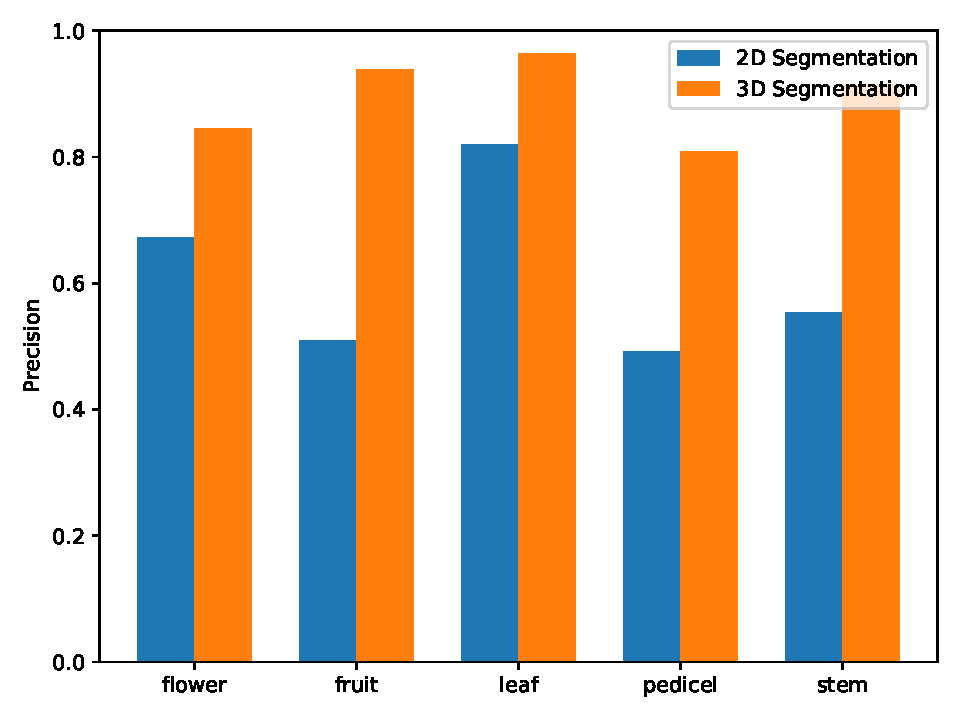
\includegraphics[width = 0.5\linewidth]{figures/eval_precision.pdf}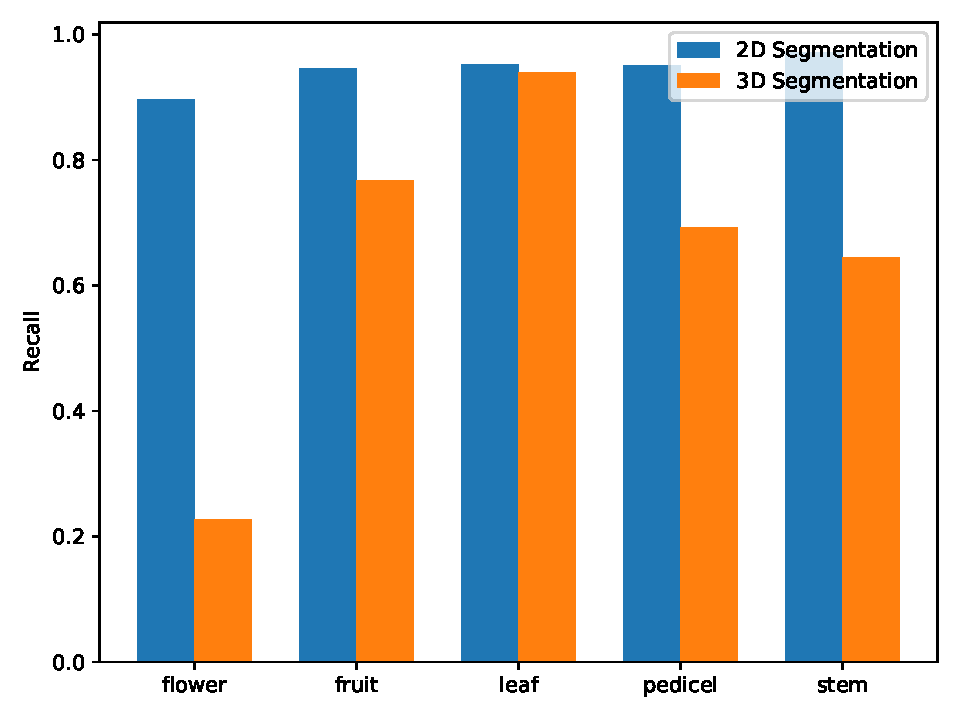
\includegraphics[width = 0.5\linewidth]{figures/eval_recall.pdf}
    \caption{Precision and recall comparison between 2D segmentation and 3D
segmentation.} \label{fig:prec_recall_2d_3d}
\end{figure}


\paragraph{2D Segmentation of real arabidopsis.}

\begin{figure}
    \centering 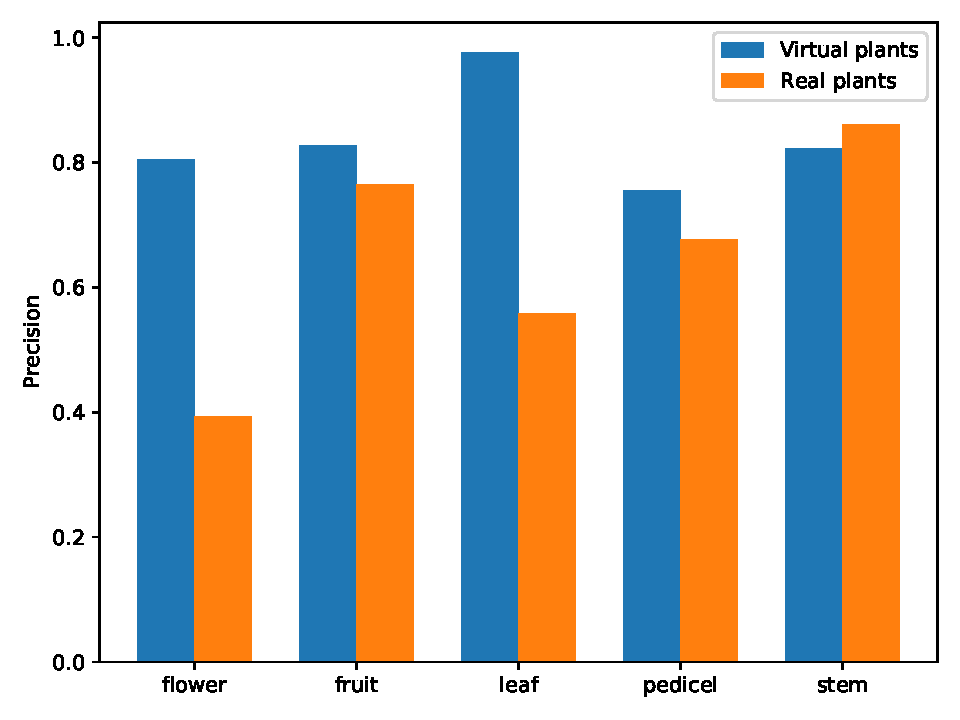
\includegraphics[width =
0.5\linewidth]{figures/eval_precision_real.pdf}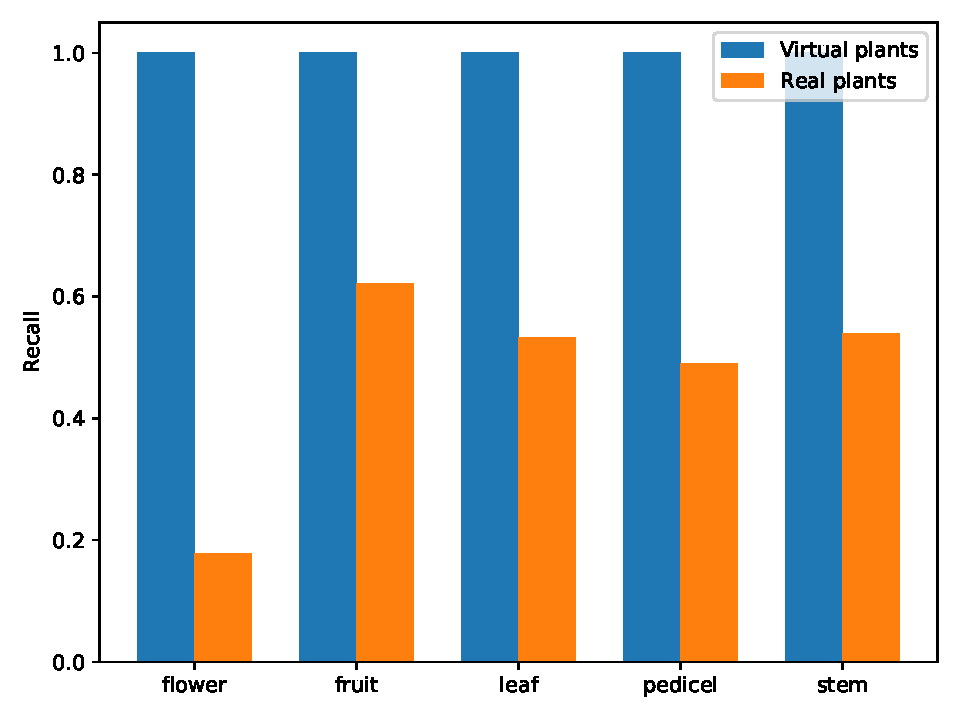
\includegraphics[width =
0.5\linewidth]{figures/eval_recall_real.pdf}
    \caption{Precision and recall comparison between 2D segmentation on
virtual and real images unseed by the neural network.} \label{fig:prec_recall_2d_3d}
\end{figure}

\paragraph{Qualitative evaluation on real plants.}

\begin{figure}
    \centering 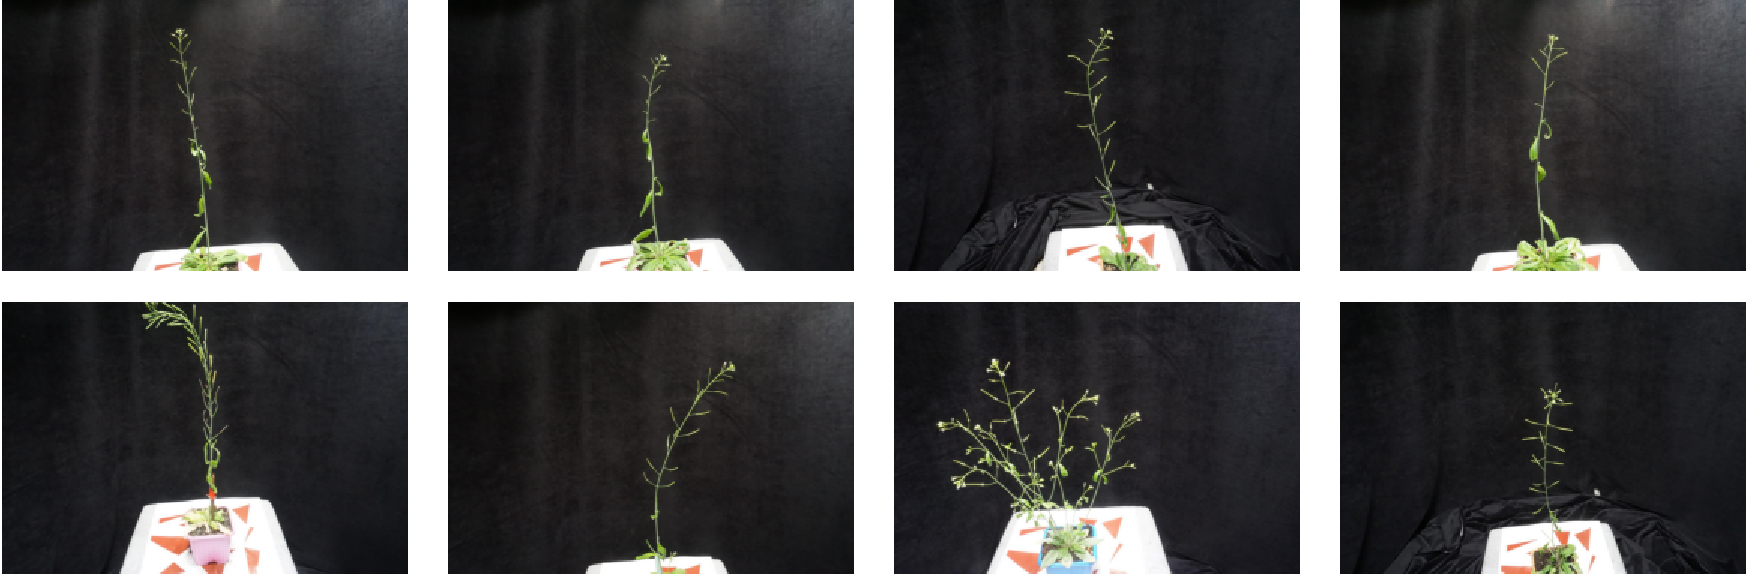
\includegraphics[width = \linewidth]{figures/seg-crop.pdf}
    \caption{Sample images from the dataset used for qualitative assessment of the method on real data} \label{fig:realscans}
\end{figure}

\begin{figure}
    \centering 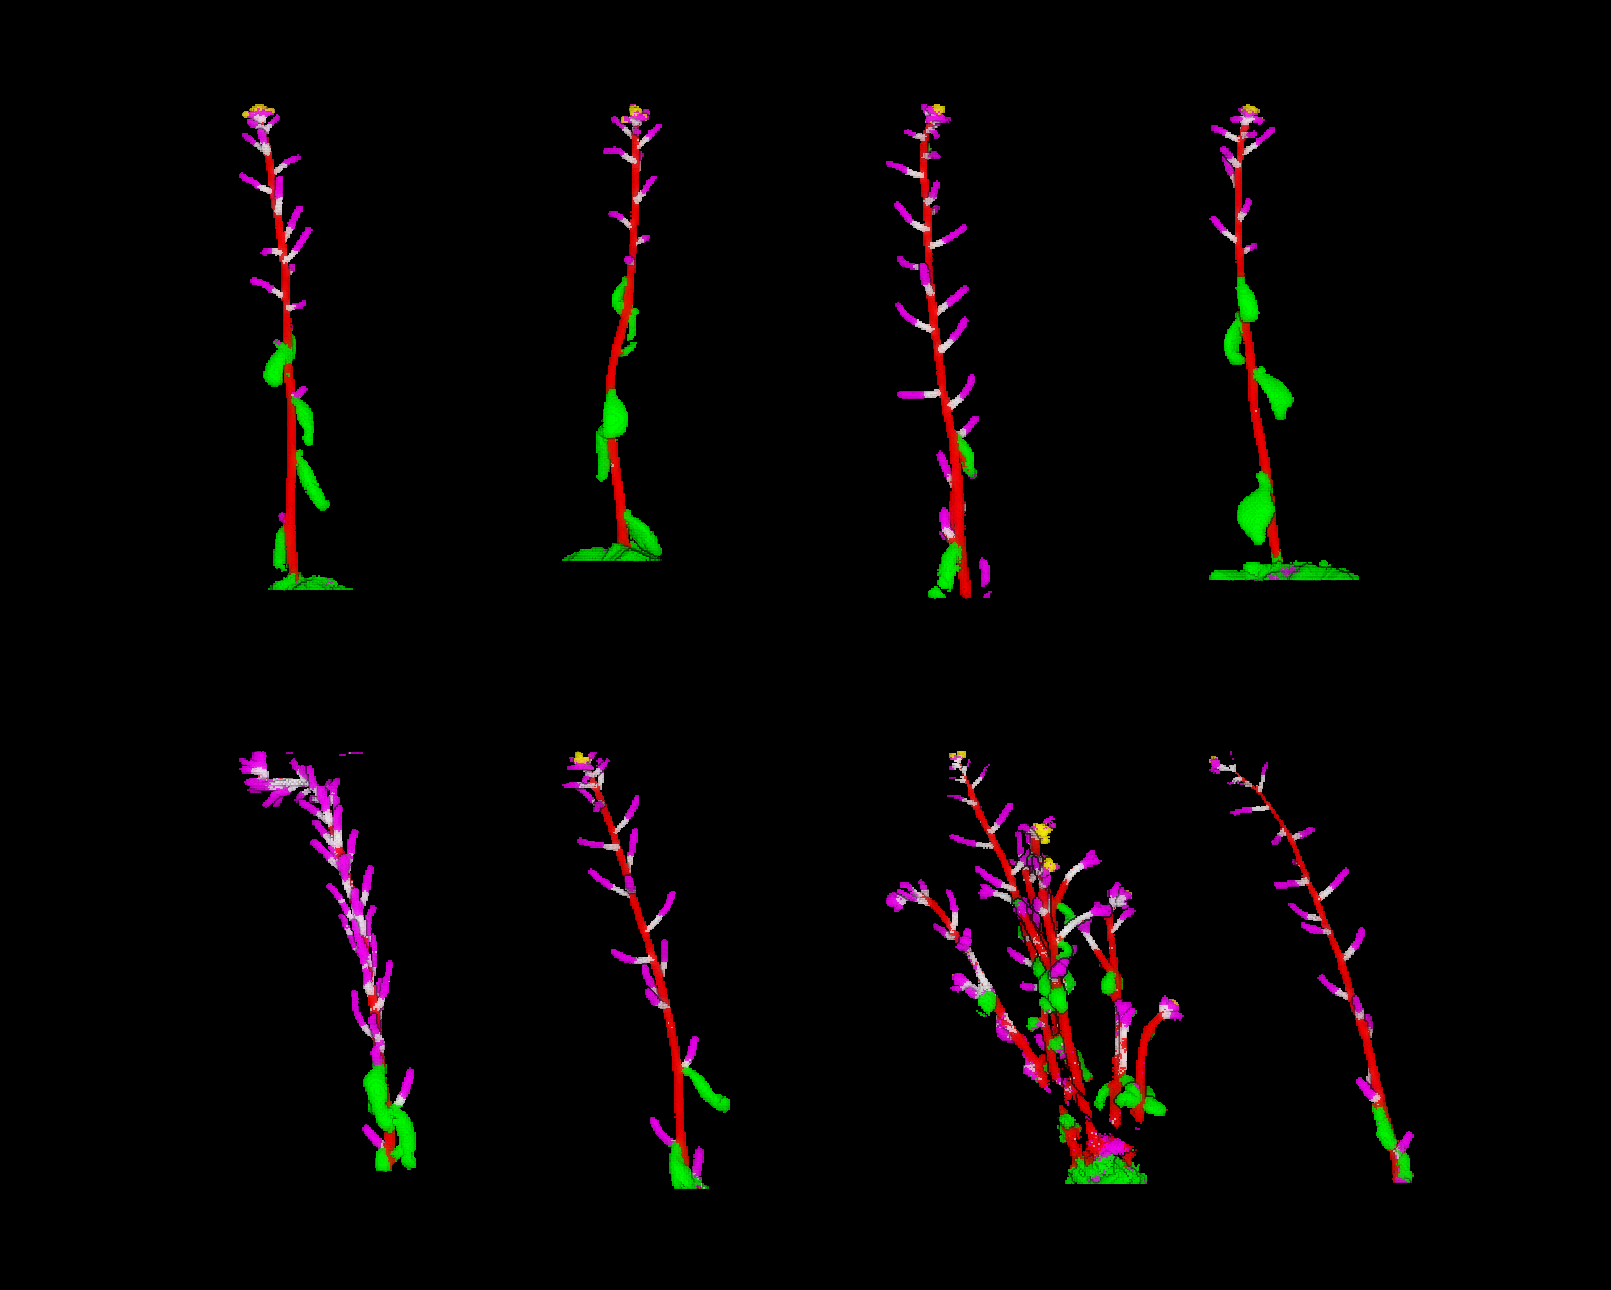
\includegraphics[width = 0.7\linewidth]{figures/capture.png}
    \caption{3D reconstruction of real plants. Red: stem, green: leaf, white: pedicel, purple: fruit:, yellow: flower} \label{fig:rec3d}
\end{figure}

\paragraph{Transfer to other species.}
To transfer to species anatomically different from \emph{A. Thaliana} we used model finetuning. This step requires a minimal number of manually annotated images (2 or 3) of the other species and allows to reconstruct the full model in 3D. To test the finetuning method we took a video turning around a tomato plant and sampled 41 images equally distributed along the video to get images from different viewpoints. Then 2 images were manually annotated with our interface. We included only the two classes present: stem and leaf. Then the network trainied on virtual \emph{A. Thaliana} was trained on these two images for 20 epochs. Then we ran the 2D segmentation (Figure \ref{fig:finetune2D}) 3D reconstruction pipeline and obtained a 3D model of the tomato.

\begin{figure}
    \centering 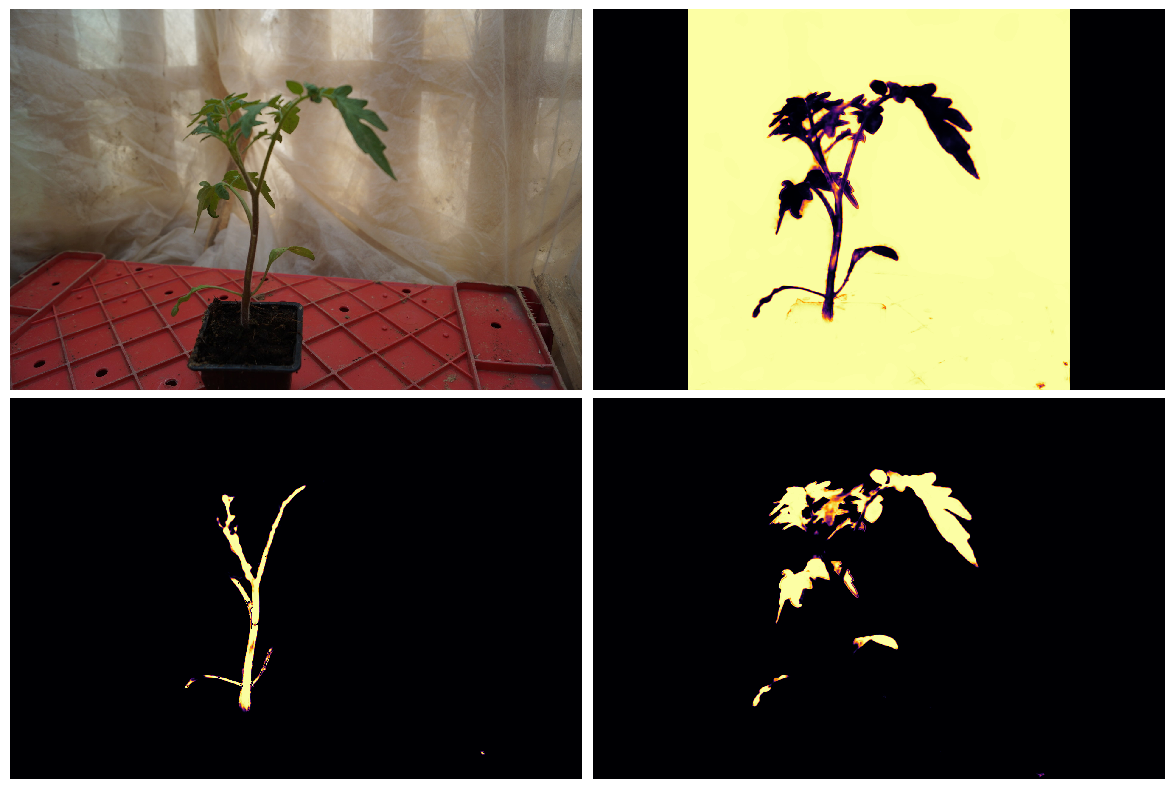
\includegraphics[width = \linewidth]{figures/finetune.png}
    \caption{Predictions of the model finetuned on two images of tomato manually annotated.} \label{fig:finetune2D}
\end{figure}


\begin{figure}
    \centering 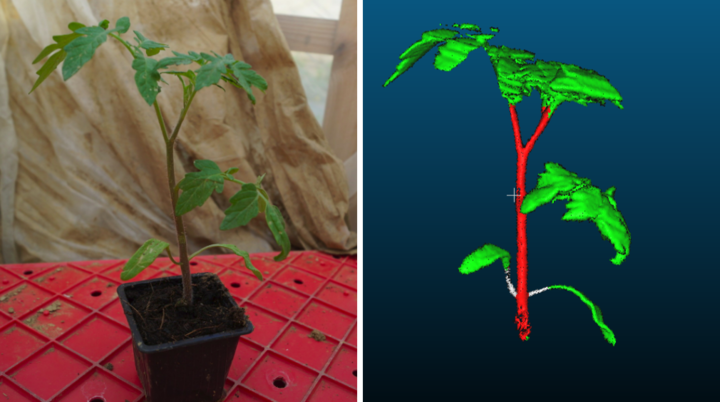
\includegraphics[width = \linewidth]{figures/tomato.png}
    \caption{3D reconstruction and segmentation of tomato plant with the pipeline.} \label{fig:finetune2D}
\end{figure}


